\documentclass[a4paper,12pt]{article}
\usepackage[utf8]{inputenc}
\usepackage[T1]{fontenc}
\usepackage[french]{babel}
\usepackage[right=2.5cm, left=2.5cm]{geometry}
\usepackage[ddmmyyyy]{datetime}
\usepackage[table]{xcolor}
\usepackage{lmodern,mathptmx,changepage,titlesec,hyperref,listings,lstautogobble,graphicx,array,longtable,multirow,lipsum,tikz,shorttoc,enumitem}
\usetikzlibrary{arrows,automata}
\usetikzlibrary{positioning}

\renewcommand{\rmdefault}{\sfdefault} %Utilisation de la police sans-serif ("Computer Modern Sans") pour la police roman
\renewcommand{\ttdefault}{pcr} 	%Utilisation d'une police "CourrierNew" pour la police monospaced (pour faire un listing manuel)
\linespread{1.15}				%Interligne

%Utilisation de liens colorés en bleu et soulignés
\hypersetup{colorlinks=true, urlcolor=blue, urlbordercolor=blue, linkcolor=black, linkbordercolor=white}
\makeatletter \Hy@AtBeginDocument{\def\@pdfborder{0 0 1} \def\@pdfborderstyle{/S/U/W 1}}\makeatother

\titlespacing*{\section} {0cm}{7ex plus 1ex minus .2ex}{1.5ex plus .2ex}
\titlespacing*{\subsection} {0cm}{4.5ex plus 1ex minus .2ex}{1.5ex plus .2ex}
\titleformat*{\section}{\huge\bfseries}
\titleformat*{\subsection}{\Large\bfseries}
\titleformat*{\subsubsection}{\normalsize\bfseries}

\definecolor{darkgreen}{rgb}{0,0.8,0}
\definecolor{mygray}{rgb}{0.93,0.93,0.93}
\definecolor{mymauve}{rgb}{0.58,0,0.82}
\lstset{	
	basicstyle=\small\ttfamily,
	backgroundcolor=\color{mygray},
	breaklines=true,
	breakatwhitespace=true,
	postbreak=\raisebox{0ex}[0ex][0ex]{\ensuremath{\color{red}\hookrightarrow\space}},
	tabsize=3,
	frame=none,
	rulecolor=\color{black},
	keywordstyle=\color{blue}\bfseries,
	stringstyle=\color{orange},
	showstringspaces=false,
	commentstyle=\footnotesize\color{darkgreen},
	keepspaces=true,
	extendedchars=true,
	numbers=left,
	numberstyle=\tiny\color{lightgray},
	stepnumber=1,
	escapeinside={(@}{@)},
	autogobble=true,
	literate=
		{á}{{\'a}}1 {é}{{\'e}}1 {í}{{}}1 {ó}{{\'o}}1 {ú}{{\'u}}1
		{Á}{{\'A}}1 {É}{{\'E}}1 {Í}{{\'I}}1 {Ó}{{\'O}}1 {Ú}{{\'U}}1
		{à}{{\`a}}1 {è}{{\`e}}1 {ì}{{\`i}}1 {ò}{{\`o}}1 {ù}{{\`u}}1
		{À}{{\`A}}1 {È}{{\'E}}1 {Ì}{{\`I}}1 {Ò}{{\`O}}1 {Ù}{{\`U}}1
		{ä}{{\"a}}1 {ë}{{\"e}}1 {ï}{{\"i}}1 {ö}{{\"o}}1 {ü}{{\"u}}1
		{Ä}{{\"A}}1 {Ë}{{\"E}}1 {Ï}{{\"I}}1 {Ö}{{\"O}}1 {Ü}{{\"U}}1
		{â}{{\^a}}1 {ê}{{\^e}}1 {î}{{\^i}}1 {ô}{{\^o}}1 {û}{{\^u}}1
		{Â}{{\^A}}1 {Ê}{{\^E}}1 {Î}{{\^I}}1 {Ô}{{\^O}}1 {Û}{{\^U}}1
		{œ}{{\oe}}1 {Œ}{{\OE}}1 {æ}{{\ae}}1 {Æ}{{\AE}}1 {ß}{{\ss}}1
		{ç}{{\c c}}1 {Ç}{{\c C}}1 {ø}{{\o}}1 {å}{{\r a}}1 {Å}{{\r A}}1
		{€}{{e}}1 {£}{{\pounds}}1 {«}{{\guillemotleft}}1
		{»}{{\guillemotright}}1 {ñ}{{\~n}}1 {Ñ}{{\~N}}1 {¿}{{?`}}1
}

%Redéfinition de la taille de \Huge pour le titre du document
\makeatletter\renewcommand\Huge{\@setfontsize\Huge{37pt}{40}}\makeatother
\date{\today}

\title{\vspace{\fill}\textbf{\Huge Manuel utilisateur}}

\begin{document}
\pagenumbering{gobble}\clearpage
\maketitle\vspace{9em}
\begin{center}
\includegraphics[scale=0.7]{../Cahier/logo.png}\end{center}
\newpage
\tableofcontents
\newpage\clearpage\pagenumbering{arabic}

\section{Introduction}
	L'applet est un outil d'analyses descriptives de données. Elle se manipule à l'aide d'un navigateur web et de fichiers \lstinline!.csv! compatibles.\\
	La navaigation entre les différentes fonctionnalités de l'applet ainsi que le format des fichiers compatibles pour les analyses sont précisées dans ce document.
	
\section{Guide Pratique}
	\subsection{Matériel nécessaire}
		Navigateur web compatible - (préciser lesquels dans quelle version plus tard)
	\subsection{Accès à l'application}
	\subsection{Étape 1-Sélection d'un fichier}
		La première fenêtre rencontrée correspond à l'index de l'application. Elle représente la première étape qui consiste à charger le fichier \lstinline!.csv! pour exécuter l'analyse descriptives de données. 
		Deux manières se présentent pour le chargement, la première consistant à faire glisser le fichier dans la zone de drop comme le montre l'illustration suivante. \\
		
	\begin{center}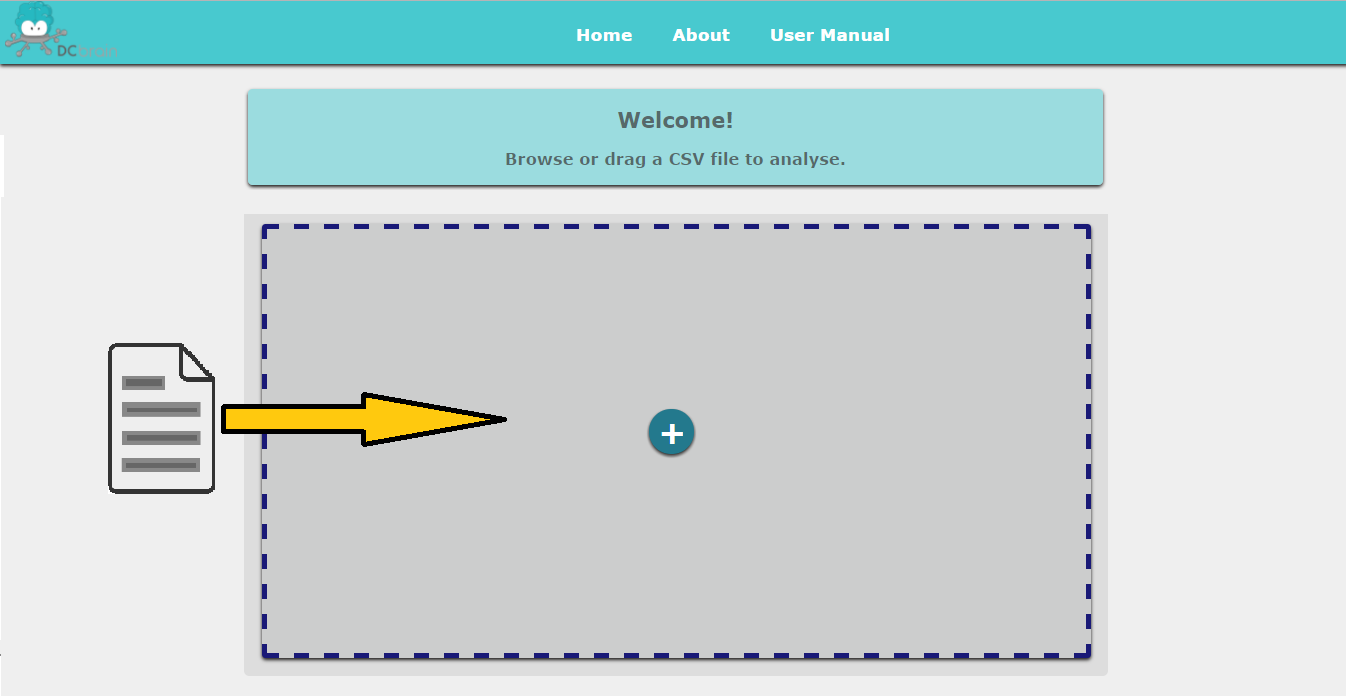
\includegraphics[scale=0.45]{fenetreDragDrop.png}\end{center}
		  
		 La seconde correspond à la méthode classique en cliquant sur le symbole \textbf{\textit{+}}, c'est à dire parcourir l'arborescence de fichiers pour trouver le document \lstinline!.csv!.\\
		 
	\begin{center}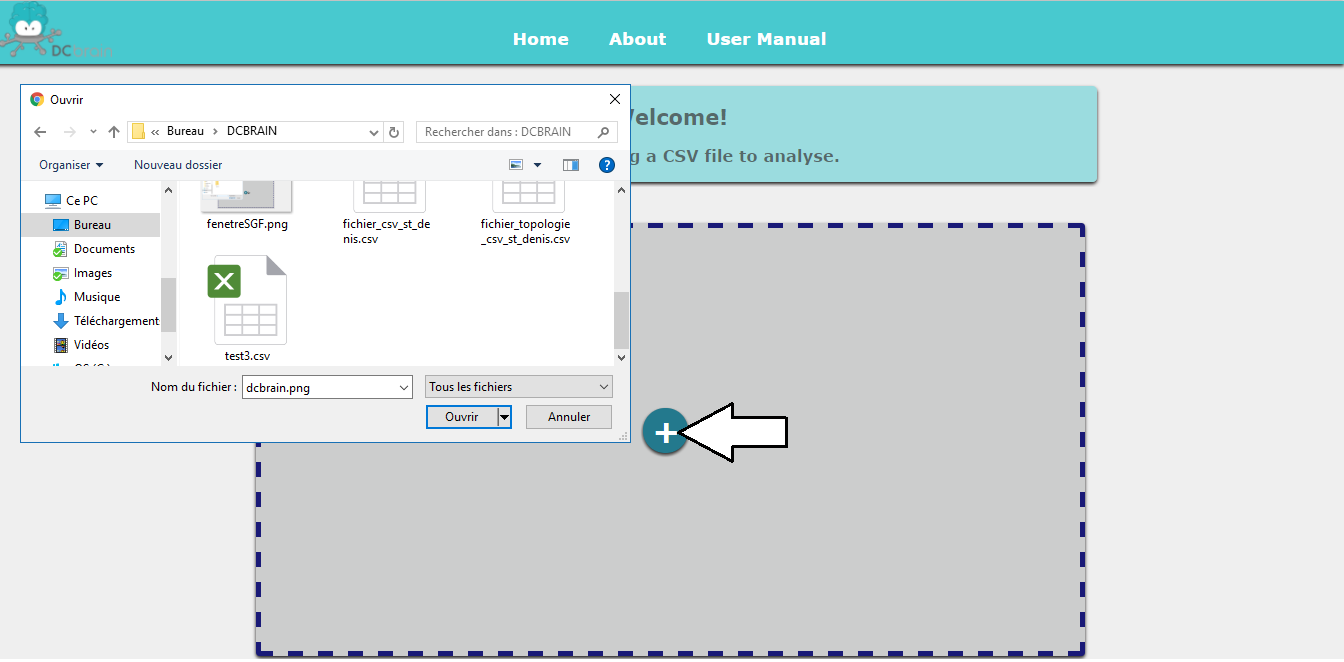
\includegraphics[scale=0.45]{fenetreSGF.png}\end{center}
	
		Les fichiers renseignés doivent décrire un format très précis pour pouvoir continuer vers la prochaine étape. Leurs contenus sont décrit par des colonnes aux types prédéfinies:
		\begin{itemize}
		\item Timestamp : jour/mois/année	\lstinline!heure:minute:seconde!
		\item Père : nom du noeud
		\item Enfant : nom du noeud
		\item Mesure (unité) : Valeur
		\end{itemize}
		Exemple :
		\begin{center}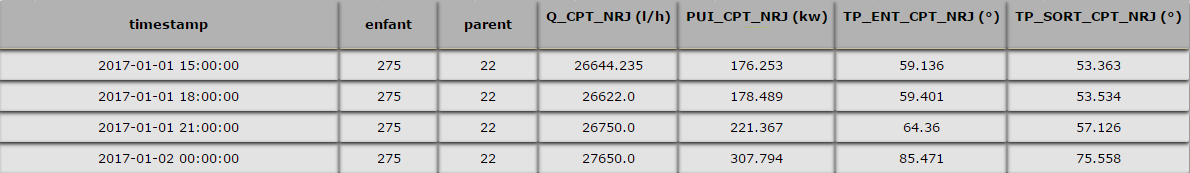
\includegraphics[scale=0.52]{exampleCSV.png}\end{center}
		
		Après avoir choisi un fichier, la page web va se rediriger vers la deuxième fenêtre de l'application si aucune erreur n'est détectées pour l'extension, l'ouverture et la lecture de ce dernier. Sinon un message d'erreur s'affiche sur la fenêtre.\\
		
				
	\begin{center}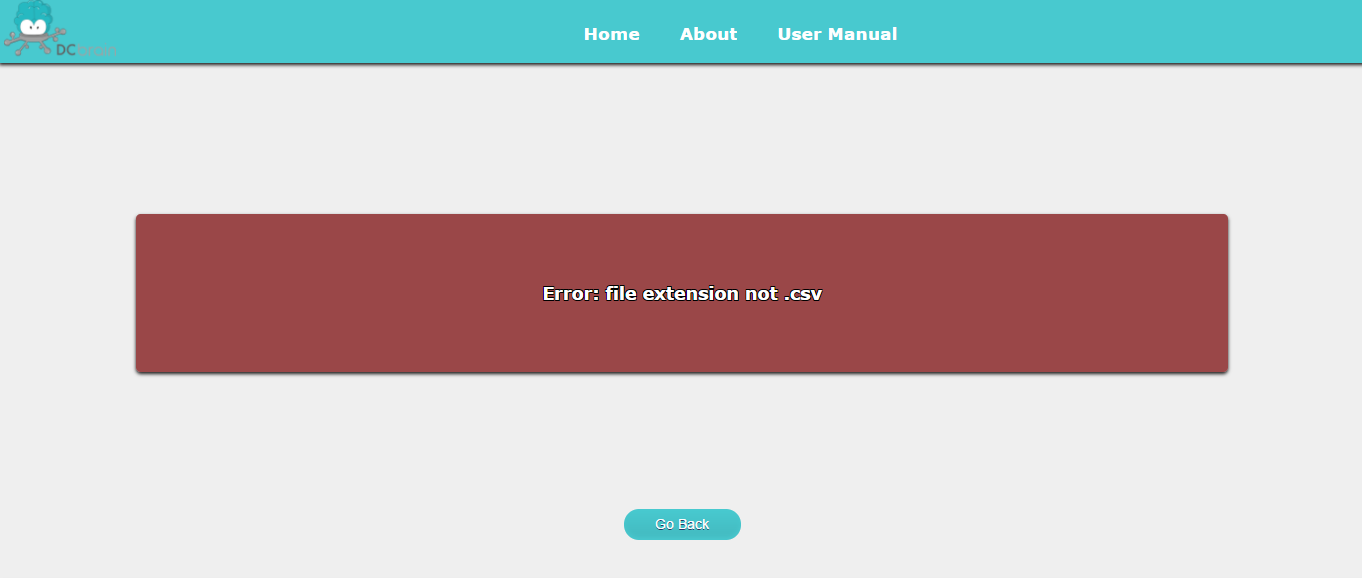
\includegraphics[scale=0.45]{fenetreErreur.png}\end{center}
			
	\subsection{Étape 2-Choix et filtrage de la colonne}
	\subsection{Étape 3-Résultats}
			\begin{center}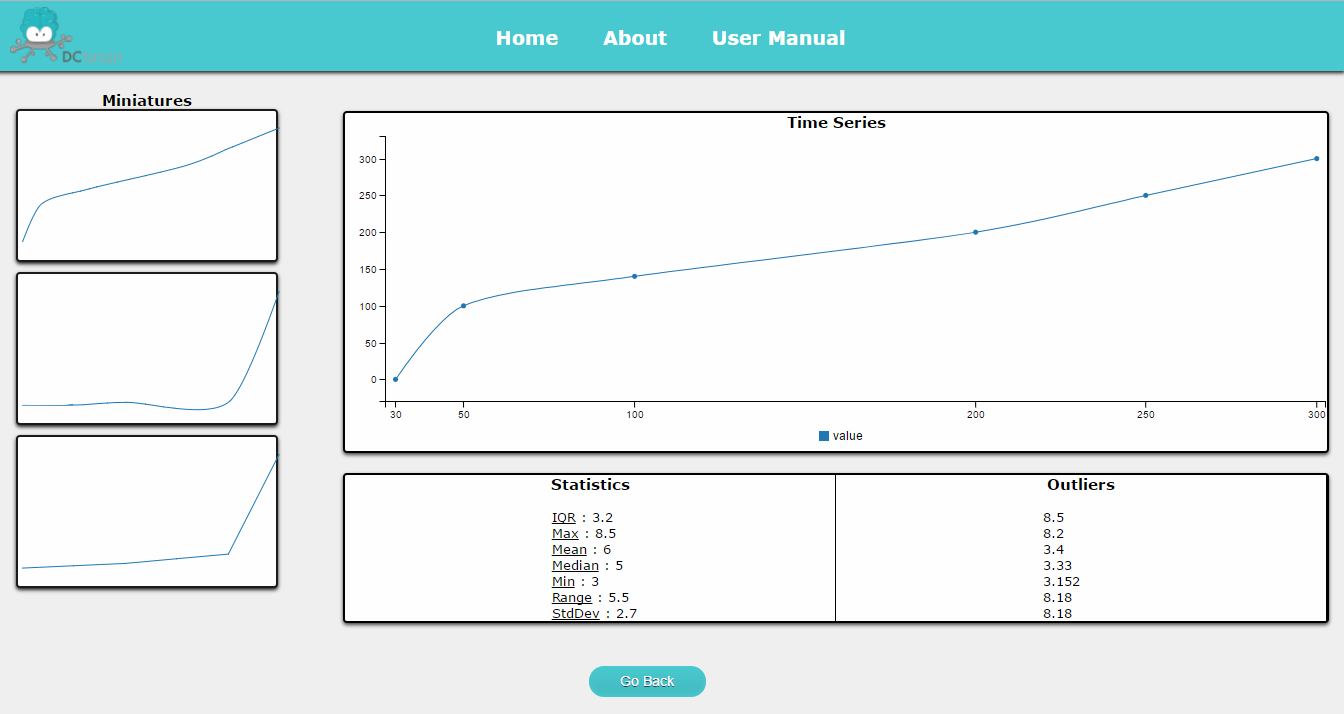
\includegraphics[scale=0.45]{fenetre3.png}\end{center}
			
		La fenêtre que vous pouvez apercevoir ci-dessus représente la dernière étape du traitement des données, l'étape de consultation des résultats d'analyse descriptive.\\
		Ces résultats sont constitués de deux catégories d'éléments :
		\begin{itemize}
			\item Des valeurs statistiques à consulter directement.
			\item Des représentations graphiques :\\
				Il suffit de cliquer sur une miniature pour accéder à une vue précise et interactive du graphe sélectionné.\\
			\begin{center}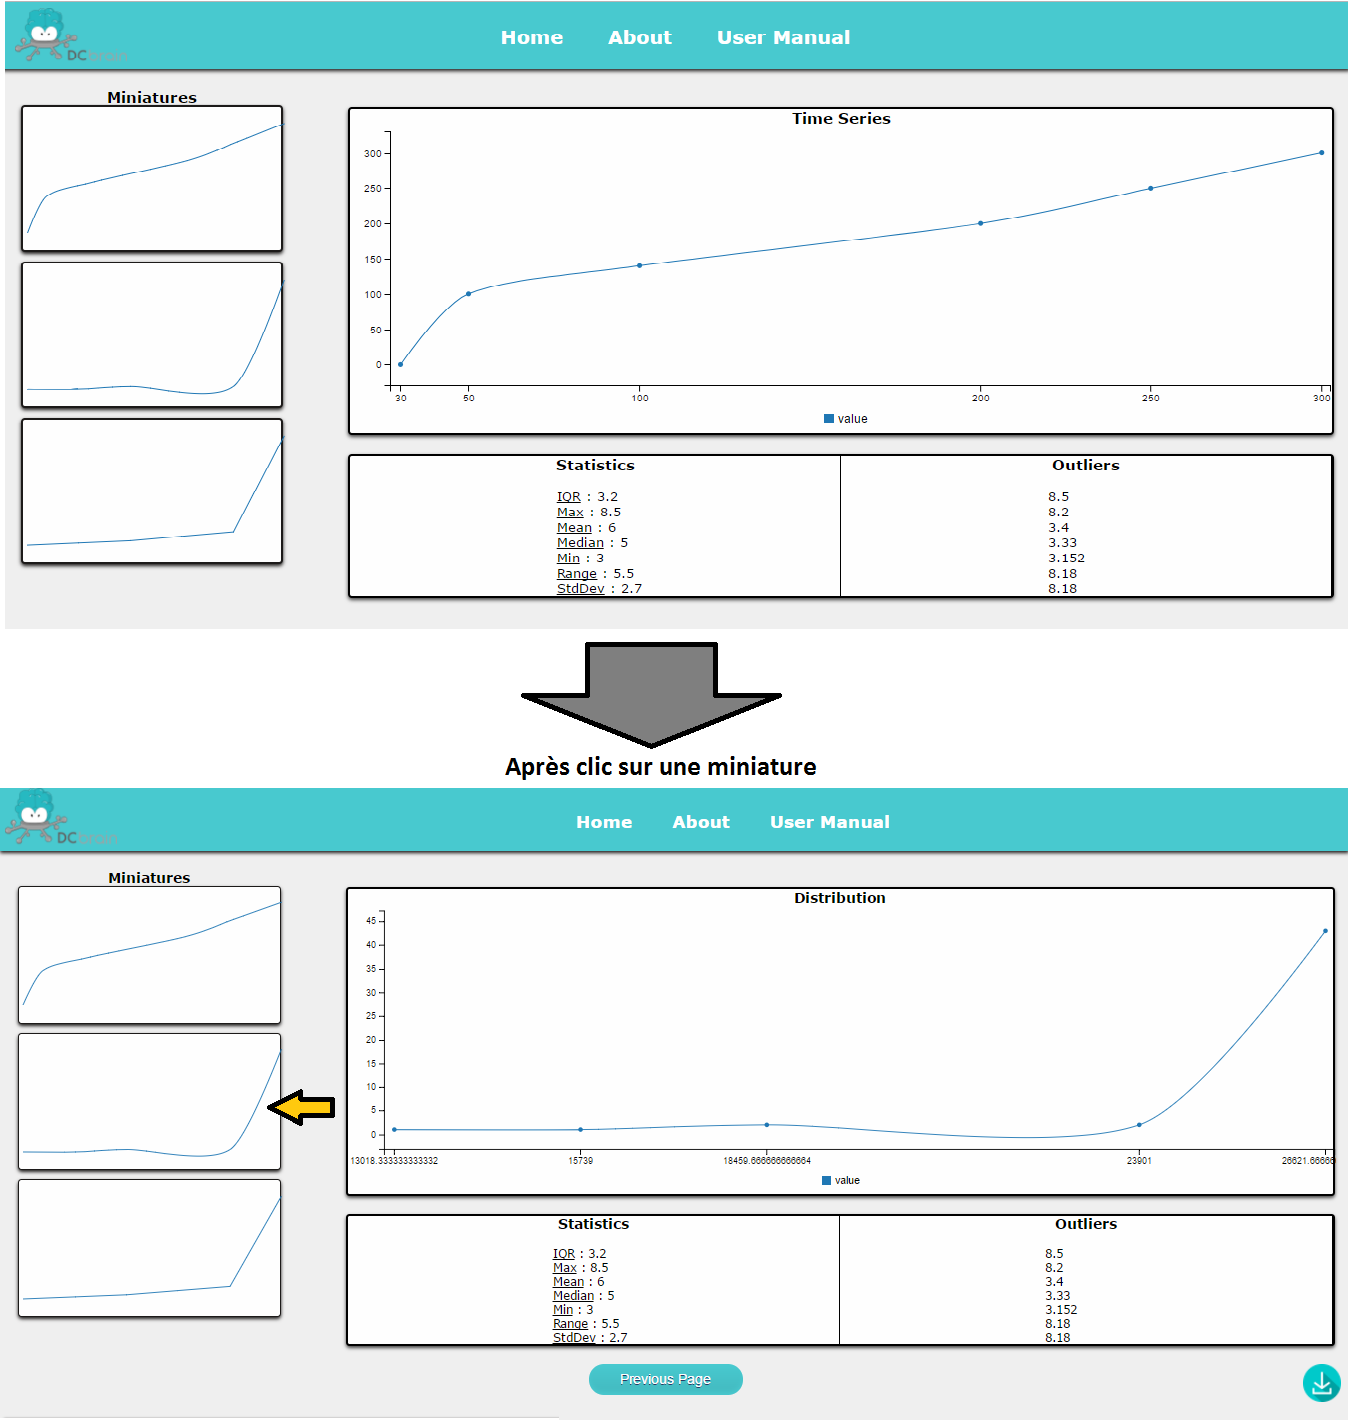
\includegraphics[scale=0.40]{fenetre3-2.png}\end{center}		
		\end{itemize}
		Finalement, une fonctionnalité de retour est disponible pour revenir à l'étape 2 et effectuer une autre analyse sans relancer l'applet du début.\\
			(Insérez un screenshot)
\end{document}
